\section{Method}
\label{sec:method}
In order to meet the initial requirements, several sensors listed below were acquired and connect to the main microcontroller.
The functionality and usage of each sensor is described in the following subsections. An ATMega2560 microcontroller
has been adapted to acquire data from the sensors and the data is constructed into a packet. A ready packet is sent to the
ESP8266 wifi module via UART. The wifi module is consisted of a microcontroller which is programmed to connect to a WiFi hotspot and
do the authentication, recognizing the packets and check the validity of the received packets. On ESP8266 one TCP client sends packets to the NodeJs server
and one HTTP server displays information such as connection status and signal strength of the module. In figure \ref{fig:arduino} a connection diagram
between these modules is represented.

A locally hosted TCP server on a PC has been developed to get weather data from the connected ESP8266 clients. In addition to
storing the data in a cloud based database, a websocket server is run and broadcasts the latest received data to all the connect users.
The users access the latest available data through WebSocket but can also fetch, filter and visualize weather data from the stored entries in the database.
The TCP server and the database have support for unlimited number of weather stations which allows the user to select a specific weather station on the browser and
study the data. In figure \ref{fig:arduino} a connection representation of the server, database and the clients is visualized.

\begin{figure}[p]
    \centering
    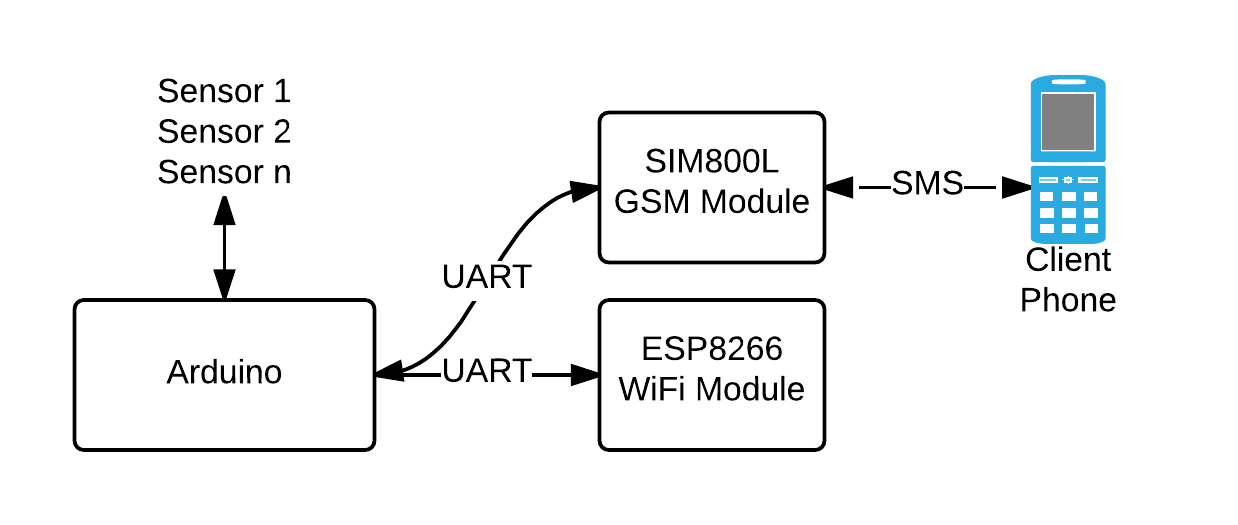
\includegraphics[width=\linewidth]{arduino}
    \caption{Arduino acquires data from the sensors periodically which are sent to the ESP8266 Wifi Module.
      The data is also available to be sent to the SIM800L module whenever requested.}
    \label{fig:arduino}
\end{figure}

\begin{figure}[p]
    \centering
    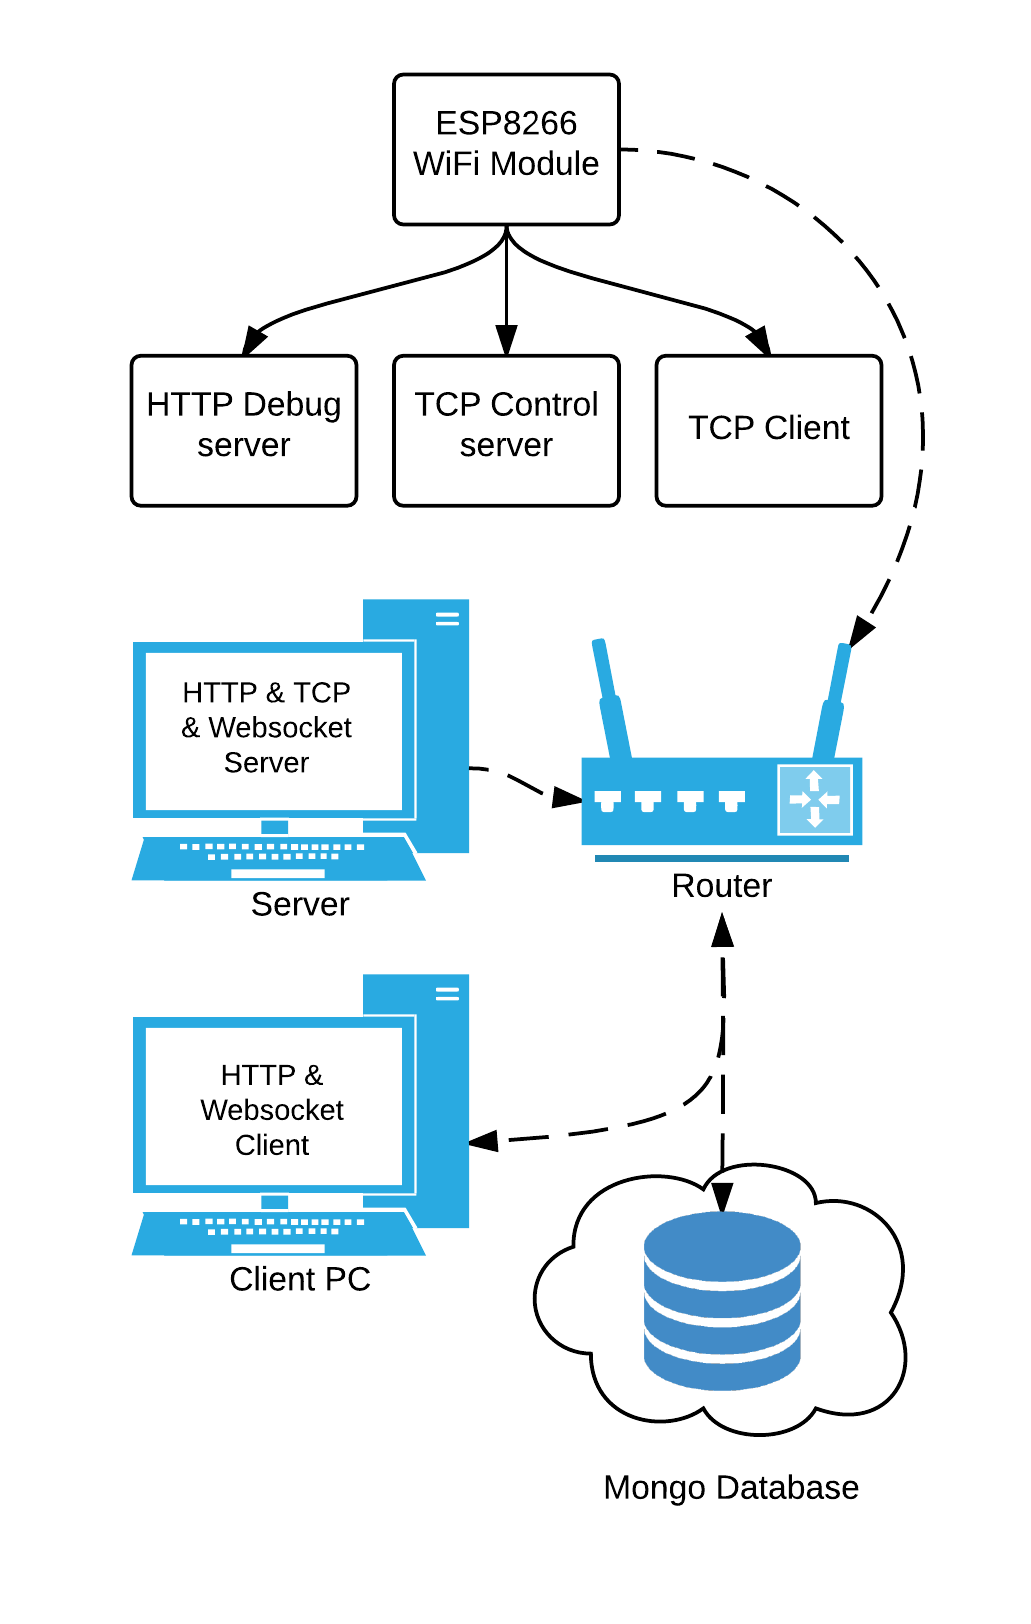
\includegraphics[width=\linewidth]{server}
    \caption{Wifi module, server and database connection diagram. Dashed line indicate wireless transmission. Arrows indicate the direction of transmission.}
    \label{fig:arduino}
\end{figure}


\subsection{Power supply (PSU)}
The subsystems require 5V respective 3.3V. With all subsystem powered on it draws around 1A.
Power supply consist of LT1086 voltage regulator which is capable of delivering 1.5A.
Two PSU was made to supply 5V respective 3.3V.
\begin{figure}[p]
    \centering
    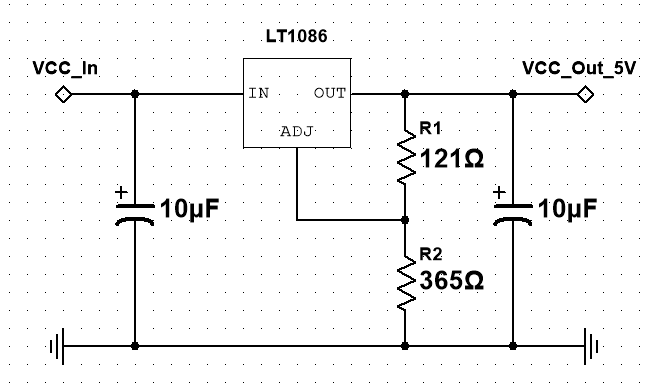
\includegraphics[width=\linewidth]{voltage_regulator}
    \caption{Voltage regulator schematic to provide with 3.3v and 5.0 volts with maximum current of 1.5A.}
    \label{fig:voltage_regulator}
\end{figure}



\subsection{UART}
For sensors which are communicating between 3.3V and 5V TTL interfaces over UART a voltage divider has been implemented.
\begin{figure}[p]
    \centering
    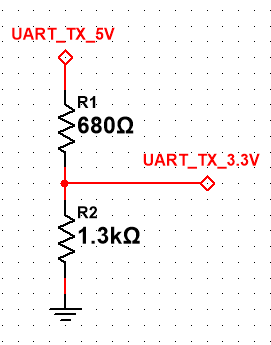
\includegraphics[height=8cm]{voltage_divider}
    \caption{Voltage divider schematic to adjust the voltage between 3.3V and 5.0V.}
    \label{fig:voltage_divider}
\end{figure}




\subsection{Packet}
Communication between Arduino, ESP8266, NodeJS server is done via custom packet of 12 Bytes data.
Since TCP checksum is only intended for the header, a custom checksum value has been added to the packet.
The overall packet consist of 2 bytes start flags, 1 bytes checksum, 1 bytes data kind, 4 bytes data value, 4 bytes timestamp.

\begin{figure}[p]
    \centering
    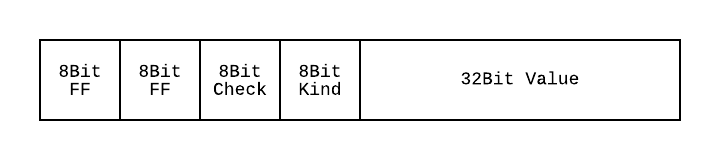
\includegraphics[width=\linewidth]{packet1}
    \caption{Custom packet structure is used for communication between Arduino, ESP8266 and the host server.}
    \label{fig:packet1}
\end{figure}


\subsection{Sensor MQ-4 and MQ-2}
Measures LPG, Methane (CH4), H2, CO, Alcohol, Smoke.
Sensor is composed by micro AL2O3 ceramic tube, Tin Dioxide (SnO2) sensitive layer,
measuring electrode and heater are fixed into a crust made by plastic and stainless steel net.


\subsection{Sensor MH-Z19 NDIR CO2}
MH-Z19 NDIR infrared gas module is a common type, small size sensor, using non-dispersive
infrared (NDIR) principle to detect the existence of CO 2 in the air, with good selectivity, non-oxygen
dependent and long life. Built-in temperature sensor can do temperature compensation; and it has
digital output and analog voltage output. It is developed by the tight integration of mature infrared absorbing
gas detection technology, precision optical circuit design and superior.

By sending the following bytes (0xFF, 0x01, 0x86, 0x00, 0x00, 0x00, 0x00, 0x00, 0x79) to the sensor via UART an response array of bytes consisting of
(Starting byte, command, High level, Low level, -, -, -, -, -, checksum) is received. Equation \ref{equ:gasConcentration} is used for conversion of the response to a PPM integer value.
The rest is of the return values is ignored.
\begin{equation}
  A_{Gas concentration} (PPM) = B_{high level} * 256 + C_{low level}
  \label{equ:gasConcentration}
\end{equation}


\subsection{Sensor GY-NEO6MV2-GPS}
The NEO-6 module series is a family of stand-alone GPS receivers featuring the high performance u-blox 6
positioning engine. These flexible and cost effective receivers offer numerous connectivity options in a miniature
16 x 12.2 x 2.4 mm package. Their compact architecture and power and memory options make NEO-6 modules
ideal for battery operated mobile devices with very strict cost and space constraints.
The 50-channel u-blox 6 positioning engine boasts a Time-To-First-Fix (TTFF) of under 1 second. The dedicated
acquisition engine, with 2 million correlators, is capable of massive parallel time/frequency space searches,
enabling it to find satellites instantly. Innovative design and technology suppresses jamming sources and
mitigates multipath effects, giving NEO-6 GPS receivers excellent navigation performance even in the most
challenging environments.

\begin{figure*}[t!]
    \centering
    \begin{subfigure}[t]{0.3\textwidth}
      \centering
      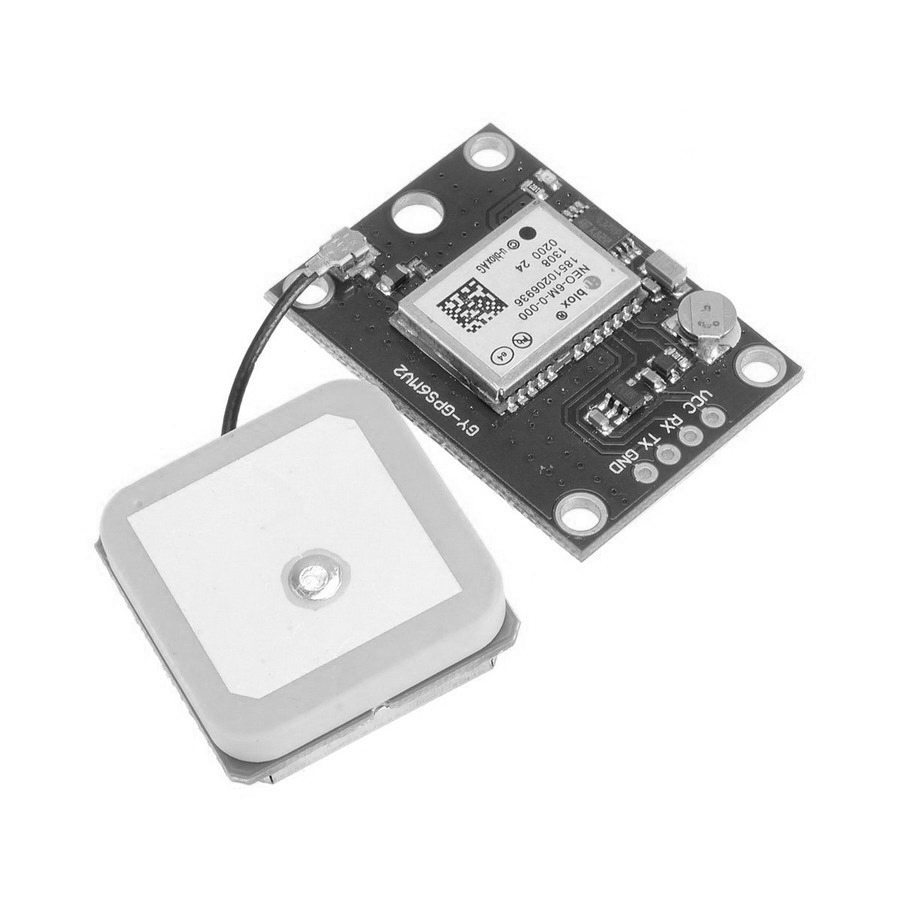
\includegraphics[height=1.5in]{GY-NEO6MV2-GPS}
      \caption{GY-NEO6MV2 GPS sensor.}
      \label{fig:GY-NEO6MV2-GPS}
    \end{subfigure}
    ~
    \begin{subfigure}[t]{0.3\textwidth}
        \centering
        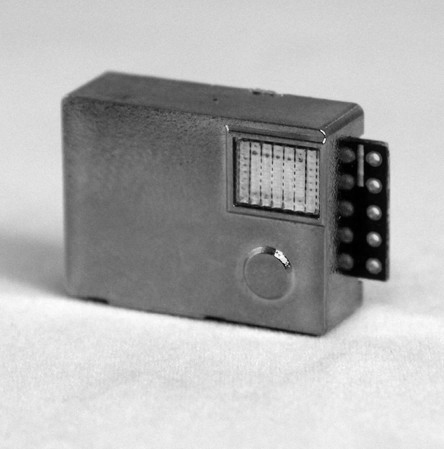
\includegraphics[height=1.5in]{MH-Z19.jpg}
        \caption{MH-Z19 CO2 sensor.}
        \label{fig:MH-Z19}
    \end{subfigure}
    ~
    \begin{subfigure}[t]{0.3\textwidth}
        \centering
        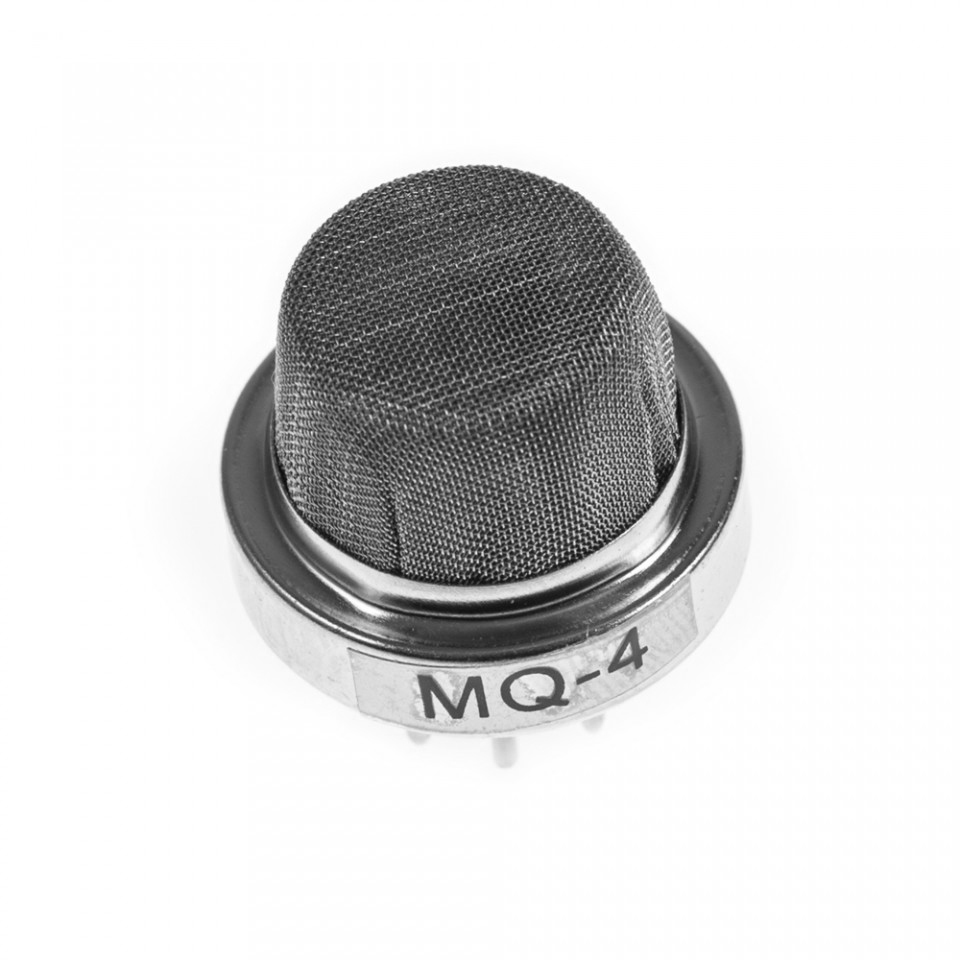
\includegraphics[height=1.5in]{MQ4}
        \caption{MQ4 gas sensor. All sensors in the MQ series have an identical appearance. }
        \label{fig:MQ4}
    \end{subfigure}
    \caption{Various sensors are used to sense the environment. }
\end{figure*}


\subsection{Thunder prediction}
The barometric pressure and thunder are hight associated to each other in a way that falling barometric pressure may result in
deteriorating weather or some form of precipitation such as wet and/or windy conditions and thunder in hot weather. As a
storm approaches air pressure begins to
fall and this can happen very quickly. Rising barometric pressure is a good indicator that no storms are developing in the
following 24 hrs and there will be fair weather or no precipitation \cite{thunder}.

\subsection{Clouds status}
In order to sense to which extent the clouds are covering the sky, satellite imagery is used. However, using a UV sensor in addition to a photosensor we are able to
detect wether its sunny or cloudy. On average, clouds do reduce the amount of ultraviolet A and B radiation that reaches the Earth's surface, but it far from stops all rays. Indeed, clouds are generally better at blocking visible light than UV.
However this method is not reliable as there might be only one cloud covering the sunlight and the rest of the sky is clear blue.

\subsection{Solar and lunar times}
There are several planetary equations to calculate set and rise times of moon and the sun or any other star.
To give one example for the sunrise, we have equation \ref{equ:sunrise}
\begin{equation}
  cos(\omega) = -tan(\phi) * tan (\delta)
  \label{equ:sunrise}
\end{equation}
where
\begin{itemize}
  \item $\omega$ is the hour angle in degrees at either sunrise (when negative value is taken) or sunset.
  \item $\phi$ is the latitude of the observer on the Earth in degrees.
  \item $\delta$ is the sun declination in degrees
\end{itemize}

The method of calculations for other paramethers is in a similar fashion. However this is out of the scope of this project and
to get more information please visit the website of Earth System Research Laboratory\footnote{http://www.esrl.noaa.gov/gmd/grad/solcalc/}.
